\documentclass{article}

% content/resources/templates/preamble.tex
\usepackage[margin=0.6in]{geometry}
\author{Milav Dabgar}
\usepackage{amsmath,amssymb,amsthm}
\usepackage{booktabs}
\usepackage{multirow}
\usepackage{xcolor}
\usepackage{tcolorbox}
\tcbuselibrary{breakable,skins}
\usepackage[colorlinks=true,linkcolor=blue]{hyperref}
\usepackage{titlesec}
\usepackage{enumitem}
\usepackage{tikz}
\usepackage{pgfplots}
\usepackage{circuitikz}
\usepackage[version=4]{mhchem}
\usepackage{longtable}
\usepackage{array}
\usepackage{float}
\usepackage{caption}
\usepackage{listings}

\lstset{
  basicstyle=\small\ttfamily,
  breaklines=true,
  breakatwhitespace=false,
  postbreak=\mbox{\textcolor{red}{$\hookrightarrow$}\space},
  float=false,
  numbers=left,
  numberstyle=\tiny\color{gray},
  numbersep=10pt,
  xleftmargin=2em,
  keywordstyle=\color{blue},
  commentstyle=\color{green!60!black},
  stringstyle=\color{purple},
  backgroundcolor=\color{gray!5},
  showstringspaces=false,
  tabsize=2,
  captionpos=b,
  keepspaces=true,
  columns=flexible
}

\pgfplotsset{compat=1.18}
\usetikzlibrary{shapes,arrows,positioning,calc,patterns,decorations.pathmorphing,decorations.markings,arrows.meta}

% Color scheme
\definecolor{headcolor}{RGB}{0,102,204}
\definecolor{keycolor}{RGB}{220,20,60}
\definecolor{solutioncolor}{RGB}{34,139,34}
\definecolor{mnemoniccolor}{RGB}{148,0,211}
\definecolor{codecolor}{RGB}{0,0,100}

% Spacing
\setlength{\parskip}{3pt}
\setlist[itemize]{nosep}
\setlist[enumerate]{nosep}

% Title formatting
\titleformat{\section}{\Large\bfseries\color{headcolor}}{\thesection}{1em}{}
\titleformat{\subsection}{\large\bfseries\color{headcolor}}{\thesubsection}{1em}{}

% Pandoc tightlist compatibility
\providecommand{\tightlist}{%
  \setlength{\itemsep}{0pt}\setlength{\parskip}{0pt}}

% Pandoc longtable compatibility
\newcounter{none}
\def\thenone{}


% content/resources/templates/english-boxes.tex

% Custom environments
\newtcolorbox{solutionbox}{
 breakable,
 enhanced,
 colback=solutioncolor!5!white,
 colframe=solutioncolor!75!black,
 fonttitle=\bfseries,
 title=Solution
}

\newtcolorbox{solutionboxnobreak}{
 colback=solutioncolor!5!white,
 colframe=solutioncolor!75!black,
 fonttitle=\bfseries,
 title=Solution
}

\newtcolorbox{keyformula}{
 breakable,
 enhanced,
 colback=keycolor!5!white,
 colframe=keycolor!75!black,
 fonttitle=\bfseries,
 title=Key Formula
}

\newtcolorbox{mnemonicboxenv}{
 breakable,
 enhanced,
 colback=mnemoniccolor!5!white,
 colframe=mnemoniccolor!75!black,
 fonttitle=\bfseries,
 title=Mnemonic
}

\newcommand{\mnemonicbox}[1]{%
  \begin{mnemonicboxenv}
    #1
  \end{mnemonicboxenv}
}


% Custom commands for GTU solutions
% This file defines semantic commands for consistent formatting

% Question command with automatic formatting
\newcommand{\question}[2]{%
  \section*{Question #1}%
  \textbf{#2}%
}

% OR question variant
\newcommand{\questionor}[2]{%
  \section*{Question #1 OR}%
  \textbf{#2}%
}

% Proper table environment with caption
\newenvironment{answertable}[1]{%
  \begin{table}[htbp]
  \centering
  \caption{#1}
}{%
  \end{table}
}

% Proper figure environment for diagrams
\newenvironment{answerdiagram}[1]{%
  \begin{figure}[htbp]
  \centering
  \caption{#1}
}{%
  \end{figure}
}

% Semantic markup for key terms
\newcommand{\keyword}[1]{\textbf{#1}}
\newcommand{\code}[1]{\texttt{#1}}
\newcommand{\classname}[1]{\texttt{#1}}
\newcommand{\methodname}[1]{\texttt{#1}}

% Proper quotation marks
\newcommand{\mnemonic}[1]{``#1''}


\title{Software Engineering (4353202) - Summer 2025 Solution}
\date{May 14, 2025}

\begin{document}
\maketitle

\questionmarks{1(a)}{3}{Enlist Software Application Domain and explain Embedded Software}

\begin{solutionbox}
\textbf{Software Application Domains:}

\begin{center}
\captionof{table}{Software Application Domains}
\begin{tabulary}{\linewidth}{|L|L|}
\hline
\textbf{Domain} & \textbf{Description} \\ \hline
System Software & Operating systems, device drivers \\ \hline
Application Software & Word processors, games, business apps \\ \hline
Engineering/Scientific Software & CAD, simulation tools \\ \hline
Embedded Software & Real-time control systems \\ \hline
Web Applications & Browser-based applications \\ \hline
AI Software & Machine learning, expert systems \\ \hline
\end{tabulary}
\end{center}

\textbf{Embedded Software} is specialized software that runs on embedded systems with dedicated hardware. It controls specific functions in devices like washing machines, cars, and medical equipment.

\begin{itemize}
    \item \keyword{Real-time operation}: Must respond within strict time limits
    \item \keyword{Resource constraints}: Limited memory and processing power
    \item \keyword{Hardware dependency}: Closely integrated with specific hardware
\end{itemize}
\end{solutionbox}

\begin{mnemonicbox}
\mnemonic{SAEEWA: System, Application, Engineering, Embedded, Web, AI}
\end{mnemonicbox}

\questionmarks{1(b)}{4}{Explain Generic Framework activities and umbrella activities}

\begin{solutionbox}
\textbf{Generic Framework Activities:}

\begin{center}
\captionof{table}{Generic Framework Activities}
\begin{tabulary}{\linewidth}{|L|L|}
\hline
\textbf{Activity} & \textbf{Purpose} \\ \hline
Communication & Gather requirements from stakeholders \\ \hline
Planning & Define work plan and schedule \\ \hline
Modeling & Create analysis and design models \\ \hline
Construction & Code generation and testing \\ \hline
Deployment & Software delivery and support \\ \hline
\end{tabulary}
\end{center}

\textbf{Umbrella Activities:}

\begin{center}
\captionof{table}{Umbrella Activities}
\begin{tabulary}{\linewidth}{|L|L|}
\hline
\textbf{Activity} & \textbf{Purpose} \\ \hline
Project Management & Track progress and control \\ \hline
Risk Management & Identify and mitigate risks \\ \hline
Quality Assurance & Ensure software quality \\ \hline
Configuration Management & Control changes \\ \hline
Work Product Preparation & Document creation \\ \hline
\end{tabulary}
\end{center}

\begin{itemize}
    \item \keyword{Framework activities}: Core sequential activities in every project
    \item \keyword{Umbrella activities}: Continuous activities throughout project lifecycle
\end{itemize}
\end{solutionbox}

\begin{mnemonicbox}
\mnemonic{CPMCD for Framework, PRQCW for Umbrella}
\end{mnemonicbox}

\questionmarks{1(c)}{7}{Recreate the software development life cycle diagram and explain its phases}

\begin{solutionbox}
\textbf{SDLC Diagram:}

\begin{center}
\begin{tikzpicture}[node distance=2.5cm, auto]
    \node [gtu state] (req) {Requirements\\Analysis};
    \node [gtu state, right of=req] (design) {System\\Design};
    \node [gtu state, right of=design] (impl) {Implementation};
    \node [gtu state, below of=impl] (test) {Testing};
    \node [gtu state, left of=test] (deploy) {Deployment};
    \node [gtu state, left of=deploy] (maint) {Maintenance};
    
    \path [gtu arrow] (req) -- (design);
    \path [gtu arrow] (design) -- (impl);
    \path [gtu arrow] (impl) -- (test);
    \path [gtu arrow] (test) -- (deploy);
    \path [gtu arrow] (deploy) -- (maint);
    \path [gtu arrow] (maint) to [bend right=45] (req);
\end{tikzpicture}
\captionof{figure}{Software Development Life Cycle}
\end{center}

\textbf{SDLC Phases:}

\begin{center}
\captionof{table}{SDLC Phases Details}
\begin{tabulary}{\linewidth}{|L|L|L|}
\hline
\textbf{Phase} & \textbf{Activities} & \textbf{Deliverables} \\ \hline
Requirements Analysis & Gather user needs, create SRS & SRS Document \\ \hline
System Design & Architecture design, UI design & Design Document \\ \hline
Implementation & Code development, unit testing & Source Code \\ \hline
Testing & Integration, system testing & Test Reports \\ \hline
Deployment & Installation, user training & Deployed System \\ \hline
Maintenance & Bug fixes, enhancements & Updated System \\ \hline
\end{tabulary}
\end{center}

\begin{itemize}
    \item \keyword{Systematic approach}: Each phase has specific inputs and outputs
    \item \keyword{Quality gates}: Reviews between phases ensure quality
    \item \keyword{Iterative nature}: Feedback improves subsequent cycles
\end{itemize}
\end{solutionbox}

\begin{mnemonicbox}
\mnemonic{Real Systems Implement Tests During Maintenance}
\end{mnemonicbox}

\questionmarks{1(c) OR}{7}{List software development models and explain any two models with necessary diagrams}

\begin{solutionbox}
\textbf{Software Development Models:}

\begin{center}
\captionof{table}{Software Development Models}
\begin{tabulary}{\linewidth}{|L|L|}
\hline
\textbf{Model} & \textbf{Characteristics} \\ \hline
Waterfall Model & Sequential, linear approach \\ \hline
Iterative Model & Repeated cycles of development \\ \hline
Spiral Model & Risk-driven, iterative \\ \hline
Agile Model & Flexible, customer collaboration \\ \hline
RAD Model & Rapid prototyping \\ \hline
V-Model & Verification and validation focus \\ \hline
\end{tabulary}
\end{center}

\textbf{1. Waterfall Model:}

\begin{center}
\begin{tikzpicture}[node distance=2cm, auto]
    \node [gtu block] (req) {Requirements};
    \node [gtu block, right of=req] (design) {Design};
    \node [gtu block, right of=design] (impl) {Implementation};
    \node [gtu block, below of=impl] (test) {Testing};
    \node [gtu block, left of=test] (deploy) {Deployment};
    \node [gtu block, left of=deploy] (maint) {Maintenance};
    
    \path [gtu arrow] (req) -- (design);
    \path [gtu arrow] (design) -- (impl);
    \path [gtu arrow] (impl) -- (test);
    \path [gtu arrow] (test) -- (deploy);
    \path [gtu arrow] (deploy) -- (maint);
\end{tikzpicture}
\captionof{figure}{Waterfall Model}
\end{center}

\textbf{2. Spiral Model:}

\begin{center}
\begin{tikzpicture}[node distance=2.5cm, auto]
    \node [gtu state] (plan) {Planning};
    \node [gtu state, right of=plan] (risk) {Risk\\Analysis};
    \node [gtu state, below of=risk] (eng) {Engineering};
    \node [gtu state, left of=eng] (eval) {Evaluation};
    
    \path [gtu arrow] (plan) -- (risk);
    \path [gtu arrow] (risk) -- (eng);
    \path [gtu arrow] (eng) -- (eval);
    \path [gtu arrow] (eval) -- (plan);
\end{tikzpicture}
\captionof{figure}{Spiral Model}
\end{center}

\begin{itemize}
    \item \keyword{Waterfall}: Simple, suitable for well-understood requirements
    \item \keyword{Spiral}: Handles high-risk projects with iterative risk assessment
\end{itemize}
\end{solutionbox}

\begin{mnemonicbox}
\mnemonic{WIRRAV: Waterfall, Iterative, RAD, Risk-driven, Agile, V-model}
\end{mnemonicbox}

\questionmarks{2(a)}{3}{Differentiate SCRUM Agile process model with SPIRAL process model}

\begin{solutionbox}
\begin{center}
\captionof{table}{SCRUM vs SPIRAL}
\begin{tabulary}{\linewidth}{|L|L|L|}
\hline
\textbf{Aspect} & \textbf{SCRUM} & \textbf{SPIRAL} \\ \hline
Approach & Agile, iterative & Risk-driven, iterative \\ \hline
Duration & Fixed sprints (2-4 weeks) & Variable spiral cycles \\ \hline
Focus & Customer collaboration & Risk management \\ \hline
Planning & Sprint planning & Comprehensive planning \\ \hline
Documentation & Minimal documentation & Detailed documentation \\ \hline
Team Size & Small teams (5-9 members) & Any team size \\ \hline
\end{tabulary}
\end{center}

\begin{itemize}
    \item \keyword{SCRUM}: Emphasizes rapid delivery and customer feedback
    \item \keyword{SPIRAL}: Focuses on risk identification and mitigation
\end{itemize}
\end{solutionbox}

\begin{mnemonicbox}
\mnemonic{SCRUM=Speed, SPIRAL=Safety}
\end{mnemonicbox}

\questionmarks{2(b)}{4}{List requirement gathering techniques and explain anyone}

\begin{solutionbox}
\textbf{Requirement Gathering Techniques:}

\begin{center}
\captionof{table}{Requirement Gathering Techniques}
\begin{tabulary}{\linewidth}{|L|L|}
\hline
\textbf{Technique} & \textbf{Description} \\ \hline
Interviews & Direct conversation with stakeholders \\ \hline
Questionnaires & Structured written questions \\ \hline
Observation & Watch users perform tasks \\ \hline
Document Analysis & Review existing documents \\ \hline
Prototyping & Build working models \\ \hline
Brainstorming & Group idea generation \\ \hline
\end{tabulary}
\end{center}

\textbf{Interview Technique Explained:}

\begin{itemize}
    \item \keyword{Structured interviews}: Predetermined questions, formal approach
    \item \keyword{Unstructured interviews}: Open-ended discussion, flexible
    \item \keyword{Semi-structured}: Combination of both approaches
\end{itemize}

\textbf{Benefits}: Direct stakeholder input, clarification possible, detailed information

\textbf{Challenges}: Time-consuming, interviewer bias, incomplete information
\end{solutionbox}

\begin{mnemonicbox}
\mnemonic{IQDPBB: Interview, Questionnaire, Document, Prototype, Brainstorm, Observe}
\end{mnemonicbox}

\questionmarks{2(c)}{7}{Define use case diagram. Explain it with example}

\begin{solutionbox}
\textbf{Use Case Diagram Definition:}

A use case diagram shows the functional requirements of a system by depicting actors and their interactions with use cases.

\textbf{Components:}

\begin{center}
\captionof{table}{Use Case Diagram Components}
\begin{tabulary}{\linewidth}{|L|L|L|}
\hline
\textbf{Component} & \textbf{Symbol} & \textbf{Purpose} \\ \hline
Actor & Stick figure & External entity \\ \hline
Use Case & Oval & System function \\ \hline
Association & Line & Actor-use case relationship \\ \hline
System Boundary & Rectangle & System scope \\ \hline
\end{tabulary}
\end{center}

\textbf{Example: Library Management System}

\begin{center}
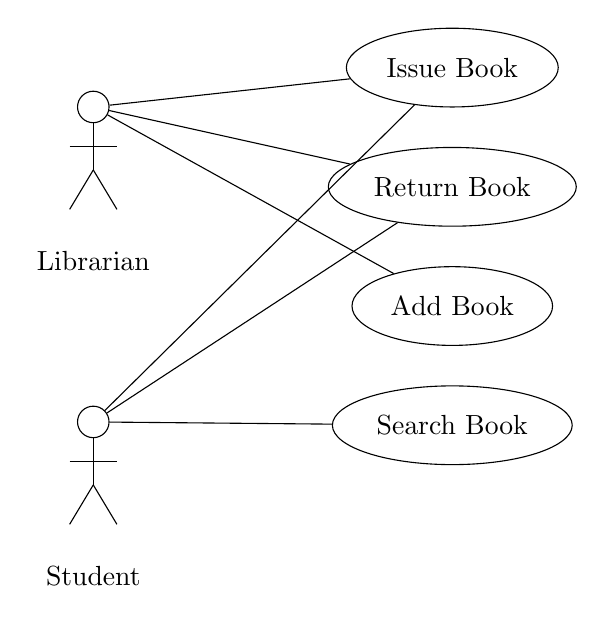
\begin{tikzpicture}[node distance=3cm, auto]
    % Actors (using simple shapes)
    \node[circle, draw, minimum size=0.4cm] (lib-head) at (0,0) {};
    \draw (0,-0.2) -- (0,-0.8);
    \draw (-0.3,-0.5) -- (0.3,-0.5);
    \draw (0,-0.8) -- (-0.3,-1.3);
    \draw (0,-0.8) -- (0.3,-1.3);
    \node[below=1.5cm of lib-head] {Librarian};
    
    \node[circle, draw, minimum size=0.4cm] (stu-head) at (0,-4) {};
    \draw (0,-4.2) -- (0,-4.8);
    \draw (-0.3,-4.5) -- (0.3,-4.5);
    \draw (0,-4.8) -- (-0.3,-5.3);
    \draw (0,-4.8) -- (0.3,-5.3);
    \node[below=1.5cm of stu-head] {Student};
    
    % Use cases
    \node [draw, ellipse, minimum width=2.5cm, minimum height=1cm, right=3cm of lib-head, yshift=0.5cm] (issue) {Issue Book};
    \node [draw, ellipse, minimum width=2.5cm, minimum height=1cm, below=0.5cm of issue] (return) {Return Book};
    \node [draw, ellipse, minimum width=2.5cm, minimum height=1cm, below=0.5cm of return] (add) {Add Book};
    \node [draw, ellipse, minimum width=2.5cm, minimum height=1cm, below=0.5cm of add] (search) {Search Book};
    
    % Associations
    \draw (lib-head) -- (issue);
    \draw (lib-head) -- (return);
    \draw (lib-head) -- (add);
    \draw (stu-head) -- (issue);
    \draw (stu-head) -- (return);
    \draw (stu-head) -- (search);
\end{tikzpicture}
\captionof{figure}{Library Management System Use Case Diagram}
\end{center}

\textbf{Relationships:}

\begin{itemize}
    \item \keyword{Include}: Common functionality shared by use cases
    \item \keyword{Extend}: Optional functionality added to base use case
    \item \keyword{Generalization}: Inheritance between actors or use cases
\end{itemize}

\textbf{Benefits}: Clear functional overview, communication tool, basis for testing
\end{solutionbox}

\begin{mnemonicbox}
\mnemonic{Actors Use Cases Inside Systems}
\end{mnemonicbox}


\questionmarks{2(a) OR}{3}{Compare Water fall model and Iterative waterfall model}

\begin{solutionbox}
\begin{center}
\captionof{table}{Waterfall vs Iterative Waterfall}
\begin{tabulary}{\linewidth}{|L|L|L|}
\hline
\textbf{Aspect} & \textbf{Waterfall Model} & \textbf{Iterative Waterfall} \\ \hline
Phases & Sequential, one-time & Repeated in iterations \\ \hline
Feedback & At end of project & After each iteration \\ \hline
Risk & High risk detection late & Early risk identification \\ \hline
Flexibility & Rigid, no changes & Accommodates changes \\ \hline
Testing & After development & Continuous testing \\ \hline
Delivery & Single final delivery & Multiple incremental deliveries \\ \hline
\end{tabulary}
\end{center}

\begin{itemize}
    \item \keyword{Waterfall}: Suitable for stable, well-defined requirements
    \item \keyword{Iterative Waterfall}: Better for evolving requirements with feedback
\end{itemize}
\end{solutionbox}

\begin{mnemonicbox}
\mnemonic{PFRTFD: Phases, Feedback, Risk, Testing, Flexibility, Delivery}
\end{mnemonicbox}

\questionmarks{2(b) OR}{4}{Define Functional and non-Functional Requirement and give examples of both}

\begin{solutionbox}
\textbf{Functional Requirements:}

Requirements that define what the system should do - specific behaviors and functions.

\textbf{Non-Functional Requirements:}

Requirements that define how the system should perform - quality attributes and constraints.

\begin{center}
\captionof{table}{Functional vs Non-Functional Requirements}
\begin{tabulary}{\linewidth}{|L|L|L|}
\hline
\textbf{Type} & \textbf{Functional} & \textbf{Non-Functional} \\ \hline
Definition & System behavior & System quality \\ \hline
Examples & Login, Calculate, Store & Performance, Security \\ \hline
Testing & Black-box testing & Load, stress testing \\ \hline
Documentation & Use cases, scenarios & Quality metrics \\ \hline
\end{tabulary}
\end{center}

\textbf{Functional Examples:}

\begin{itemize}
    \item User authentication and login
    \item Calculate total bill amount
    \item Generate monthly reports
\end{itemize}

\textbf{Non-Functional Examples:}

\begin{itemize}
    \item System response time $<$ 2 seconds (Performance)
    \item 99.9\% system availability (Reliability)
    \item Support 1000 concurrent users (Scalability)
\end{itemize}
\end{solutionbox}

\begin{mnemonicbox}
\mnemonic{Functional=What, Non-Functional=How}
\end{mnemonicbox}

\questionmarks{2(c) OR}{7}{Define cohesion. Explain classification of cohesion}

\begin{solutionbox}
\textbf{Cohesion Definition:}

Cohesion measures how closely related elements within a module are. High cohesion indicates a well-designed module.

\textbf{Classification of Cohesion (Strongest to Weakest):}

\begin{center}
\captionof{table}{Types of Cohesion}
\begin{tabulary}{\linewidth}{|L|L|L|}
\hline
\textbf{Type} & \textbf{Description} & \textbf{Example} \\ \hline
Functional & Single, well-defined task & Calculate square root \\ \hline
Sequential & Output of one = input of next & Read→Process→Write \\ \hline
Communicational & Operate on same data & Update customer record \\ \hline
Procedural & Follow sequence of execution & Process payroll steps \\ \hline
Temporal & Execute at same time & System initialization \\ \hline
Logical & Similar logical functions & All input/output operations \\ \hline
Coincidental & No meaningful relationship & Random utilities \\ \hline
\end{tabulary}
\end{center}

\begin{center}
\begin{tikzpicture}[node distance=2cm, auto]
    \node [gtu block] (func) {Functional\\(Strongest)};
    \node [gtu block, right of=func] (seq) {Sequential};
    \node [gtu block, right of=seq] (comm) {Communicational};
    \node [gtu block, below of=comm] (proc) {Procedural};
    \node [gtu block, left of=proc] (temp) {Temporal};
    \node [gtu block, left of=temp] (log) {Logical};
    \node [gtu block, below of=log] (coin) {Coincidental\\(Weakest)};
    
    \path [gtu arrow] (func) -- (seq);
    \path [gtu arrow] (seq) -- (comm);
    \path [gtu arrow] (comm) -- (proc);
    \path [gtu arrow] (proc) -- (temp);
    \path [gtu arrow] (temp) -- (log);
    \path [gtu arrow] (log) -- (coin);
\end{tikzpicture}
\captionof{figure}{Cohesion Hierarchy}
\end{center}

\textbf{Goal}: Achieve functional cohesion for maintainable, reliable modules
\end{solutionbox}

\begin{mnemonicbox}
\mnemonic{Frank's Smart Cat Plays Tennis Like Crazy}
\end{mnemonicbox}

\questionmarks{3(a)}{3}{List characteristics of good software design}

\begin{solutionbox}
\textbf{Characteristics of Good Software Design:}

\begin{center}
\captionof{table}{Good Software Design Characteristics}
\begin{tabulary}{\linewidth}{|L|L|}
\hline
\textbf{Characteristic} & \textbf{Description} \\ \hline
Modularity & Divided into independent modules \\ \hline
Abstraction & Hide implementation details \\ \hline
Encapsulation & Bundle data and methods together \\ \hline
Hierarchy & Organized in layers/levels \\ \hline
Simplicity & Easy to understand and maintain \\ \hline
Flexibility & Accommodate future changes \\ \hline
\end{tabulary}
\end{center}

\begin{itemize}
    \item \keyword{High cohesion}: Related elements grouped together
    \item \keyword{Low coupling}: Minimal dependencies between modules
    \item \keyword{Reusability}: Components can be reused in other systems
\end{itemize}
\end{solutionbox}

\begin{mnemonicbox}
\mnemonic{MAEHSF: Modularity, Abstraction, Encapsulation, Hierarchy, Simplicity, Flexibility}
\end{mnemonicbox}

\questionmarks{3(b)}{4}{Explain Project Estimation Techniques using intermediate COCOMO model}

\begin{solutionbox}
\textbf{Intermediate COCOMO Model:}

Extends basic COCOMO by considering cost drivers that affect productivity.

\textbf{Formula:}

\begin{center}
\textbf{Effort = a $\times$ (KLOC)$^b$ $\times$ EAF}
\end{center}

\textbf{Cost Drivers:}

\begin{center}
\captionof{table}{COCOMO Cost Drivers}
\begin{tabulary}{\linewidth}{|L|L|L|}
\hline
\textbf{Category} & \textbf{Drivers} & \textbf{Impact} \\ \hline
Product & Reliability, Complexity & Effort multiplier \\ \hline
Hardware & Execution time, Storage & Performance constraints \\ \hline
Personnel & Analyst capability, Experience & Team skills \\ \hline
Project & Modern practices, Schedule & Development environment \\ \hline
\end{tabulary}
\end{center}

\textbf{Effort Adjustment Factor (EAF):}

EAF = Product of all cost driver multipliers

\textbf{Steps:}

\begin{enumerate}
    \item Estimate KLOC (thousands of lines of code)
    \item Select appropriate a, b values based on project type
    \item Evaluate cost drivers (scale 0.70 to 1.65)
    \item Calculate EAF
    \item Apply formula to get effort in person-months
\end{enumerate}
\end{solutionbox}

\begin{mnemonicbox}
\mnemonic{PHPP: Product, Hardware, Personnel, Project drivers}
\end{mnemonicbox}

\questionmarks{3(c)}{7}{Draw and explain level-1 Data flow diagram for Online shopping system}

\begin{solutionbox}
\textbf{Level-1 DFD for Online Shopping System:}

\begin{center}
\begin{tikzpicture}[node distance=3cm, auto]
    % External entities
    \node [draw, rectangle] (customer) {Customer};
    \node [draw, rectangle, below=4cm of customer] (payment) {Payment\\Gateway};
    \node [draw, rectangle, below=4cm of payment] (inventory) {Inventory\\Manager};
    
    % Processes
    \node [gtu block, right=3cm of customer] (order) {1.0\\Process\\Order};
    \node [gtu block, right=3cm of payment] (pay) {2.0\\Process\\Payment};
    \node [gtu block, right=3cm of inventory] (inv) {3.0\\Manage\\Inventory};
    
    % Data flows
    \path [gtu arrow] (customer) -- node[above] {Order Info} (order);
    \path [gtu arrow] (order) -- node[below] {Product Info} (customer);
    \path [gtu arrow] (order) -- node[right] {Order Details} (pay);
    \path [gtu arrow] (pay) -- node[above] {Payment Info} (payment);
    \path [gtu arrow] (payment) -- node[below] {Payment Status} (pay);
    \path [gtu arrow] (pay) -- node[right] {Inventory Update} (inv);
    \path [gtu arrow] (inv) -- node[above] {Stock Info} (inventory);
    \path [gtu arrow] (inventory) -- node[below] {Stock Status} (inv);
\end{tikzpicture}
\captionof{figure}{Level-1 DFD for Online Shopping System}
\end{center}

\textbf{Processes:}

\begin{center}
\captionof{table}{DFD Processes}
\begin{tabulary}{\linewidth}{|L|L|L|L|}
\hline
\textbf{Process} & \textbf{Input} & \textbf{Output} & \textbf{Description} \\ \hline
Process Order & Customer order & Order confirmation & Handle order placement \\ \hline
Process Payment & Payment details & Payment status & Process transactions \\ \hline
Manage Inventory & Stock queries & Stock status & Track product availability \\ \hline
\end{tabulary}
\end{center}

\textbf{Data Stores:}

\begin{itemize}
    \item \keyword{Product Database}: Store product information
    \item \keyword{Order Database}: Store order details
    \item \keyword{Customer Database}: Store customer profiles
\end{itemize}

\textbf{External Entities:}

\begin{itemize}
    \item \keyword{Customer}: Places orders, makes payments
    \item \keyword{Payment Gateway}: Processes payments
    \item \keyword{Inventory Manager}: Updates stock levels
\end{itemize}
\end{solutionbox}

\begin{mnemonicbox}
\mnemonic{PPMI: Process order, Process payment, Manage inventory}
\end{mnemonicbox}

\questionmarks{3(a) OR}{3}{Differentiate analysis and design}

\begin{solutionbox}
\begin{center}
\captionof{table}{Analysis vs Design}
\begin{tabulary}{\linewidth}{|L|L|L|}
\hline
\textbf{Aspect} & \textbf{Analysis} & \textbf{Design} \\ \hline
Focus & What system should do & How system will work \\ \hline
Phase & Requirements phase & Design phase \\ \hline
Output & Problem understanding & Solution structure \\ \hline
Models & Use cases, requirements & Architecture, classes \\ \hline
Perspective & User's viewpoint & Developer's viewpoint \\ \hline
Level & Abstract, conceptual & Concrete, detailed \\ \hline
\end{tabulary}
\end{center}

\begin{itemize}
    \item \keyword{Analysis}: Problem-focused, understanding requirements
    \item \keyword{Design}: Solution-focused, creating system architecture
\end{itemize}
\end{solutionbox}

\begin{mnemonicbox}
\mnemonic{Analysis=WHAT, Design=HOW}
\end{mnemonicbox}

\questionmarks{3(b) OR}{4}{Explain Project Estimation Techniques using basic COCOMO model}

\begin{solutionbox}
\textbf{Basic COCOMO Model:}

Estimates software development effort based on lines of code.

\textbf{Formula:}

\begin{itemize}
    \item Effort = a $\times$ (KLOC)$^b$ person-months
    \item Time = c $\times$ (Effort)$^d$ months
\end{itemize}

\textbf{Project Types:}

\begin{center}
\captionof{table}{COCOMO Project Types}
\begin{tabulary}{\linewidth}{|L|C|C|C|C|L|}
\hline
\textbf{Type} & \textbf{a} & \textbf{b} & \textbf{c} & \textbf{d} & \textbf{Description} \\ \hline
Organic & 2.4 & 1.05 & 2.5 & 0.38 & Small, experienced team \\ \hline
Semi-detached & 3.0 & 1.12 & 2.5 & 0.35 & Medium size, mixed team \\ \hline
Embedded & 3.6 & 1.20 & 2.5 & 0.32 & Complex, tight constraints \\ \hline
\end{tabulary}
\end{center}

\textbf{Steps:}

\begin{enumerate}
    \item Estimate KLOC (thousands of lines of code)
    \item Identify project type (organic/semi-detached/embedded)
    \item Apply appropriate coefficients
    \item Calculate effort and development time
\end{enumerate}

\textbf{Example}: 10 KLOC organic project

\begin{itemize}
    \item Effort = 2.4 $\times$ (10)$^{1.05}$ = 25.2 person-months
    \item Time = 2.5 $\times$ (25.2)$^{0.38}$ = 8.4 months
\end{itemize}
\end{solutionbox}

\begin{mnemonicbox}
\mnemonic{OSE: Organic, Semi-detached, Embedded}
\end{mnemonicbox}

\questionmarks{3(c) OR}{7}{Draw and explain Class Diagram for Library Management system}

\begin{solutionbox}
\textbf{Class Diagram for Library Management System:}

\begin{center}
\begin{tikzpicture}[node distance=3cm, auto]
    % Library class
    \node [draw, rectangle, minimum width=3cm, minimum height=2.5cm] (library) at (0,0) {
        \begin{tabular}{c}
        \textbf{Library} \\
        \hline
        +name: String \\
        +address: String \\
        \hline
        +addBook() \\
        +removeBook() \\
        +searchBook()
        \end{tabular}
    };
    
    % Book class
    \node [draw, rectangle, minimum width=3cm, minimum height=3cm, right=4cm of library] (book) {
        \begin{tabular}{c}
        \textbf{Book} \\
        \hline
        +bookId: String \\
        +title: String \\
        +author: String \\
        +ISBN: String \\
        +isAvailable: Boolean \\
        \hline
        +getDetails()
        \end{tabular}
    };
    
    % Member class
    \node [draw, rectangle, minimum width=3cm, minimum height=2.5cm, below=3cm of library] (member) {
        \begin{tabular}{c}
        \textbf{Member} \\
        \hline
        +memberId: String \\
        +name: String \\
        +email: String \\
        +phone: String \\
        \hline
        +issueBook() \\
        +returnBook()
        \end{tabular}
    };
    
    % Transaction class
    \node [draw, rectangle, minimum width=3cm, minimum height=2.5cm, below=3cm of book] (trans) {
        \begin{tabular}{c}
        \textbf{Transaction} \\
        \hline
        +transactionId: String \\
        +issueDate: Date \\
        +returnDate: Date \\
        +fine: Double \\
        \hline
        +calculateFine()
        \end{tabular}
    };
    
    % Relationships
    \draw [gtu arrow] (library) -- node[above] {1..*} (book);
    \draw [gtu arrow] (member) -- node[above] {1..*} (trans);
    \draw [gtu arrow] (book) -- node[right] {1..*} (trans);
\end{tikzpicture}
\captionof{figure}{Library Management System Class Diagram}
\end{center}

\textbf{Relationships:}

\begin{center}
\captionof{table}{Class Relationships}
\begin{tabulary}{\linewidth}{|L|L|L|}
\hline
\textbf{Relationship} & \textbf{Description} & \textbf{Multiplicity} \\ \hline
Library-Book & Library contains books & 1 to many \\ \hline
Member-Transaction & Member has transactions & 1 to many \\ \hline
Book-Transaction & Book involved in transactions & 1 to many \\ \hline
\end{tabulary}
\end{center}

\textbf{Key Features:}

\begin{itemize}
    \item \keyword{Attributes}: Data members of each class
    \item \keyword{Methods}: Functions that operate on class data
    \item \keyword{Associations}: Relationships between classes showing how they interact
\end{itemize}
\end{solutionbox}

\begin{mnemonicbox}
\mnemonic{LBMT: Library, Book, Member, Transaction}
\end{mnemonicbox}

\questionmarks{4(a)}{3}{List Project Size Estimation Metrics and define them}

\begin{solutionbox}
\textbf{Project Size Estimation Metrics:}

\begin{center}
\captionof{table}{Size Estimation Metrics}
\begin{tabulary}{\linewidth}{|L|L|L|}
\hline
\textbf{Metric} & \textbf{Definition} & \textbf{Usage} \\ \hline
Lines of Code (LOC) & Count of executable code lines & Traditional sizing \\ \hline
Function Points (FP) & Measure based on functionality & Language-independent \\ \hline
Feature Points & Extended function points & Real-time systems \\ \hline
Object Points & Count of objects and methods & Object-oriented systems \\ \hline
Use Case Points & Based on use case complexity & Requirements-based \\ \hline
\end{tabulary}
\end{center}

\textbf{Function Points Components:}

\begin{itemize}
    \item \keyword{External Inputs}: Data entry screens
    \item \keyword{External Outputs}: Reports, messages
    \item \keyword{External Inquiries}: Interactive queries
    \item \keyword{Internal Files}: Master files
    \item \keyword{External Interfaces}: Shared data
\end{itemize}

\textbf{Benefits}: Early estimation, technology-independent, standardized approach
\end{solutionbox}

\begin{mnemonicbox}
\mnemonic{LFFOU: LOC, Function Points, Feature Points, Object Points, Use Case Points}
\end{mnemonicbox}

\questionmarks{4(b)}{4}{Explain Risk identification in detail}

\begin{solutionbox}
\textbf{Risk Identification:}

Process of finding, recognizing, and describing potential risks that could affect project success.

\textbf{Risk Categories:}

\begin{center}
\captionof{table}{Risk Categories}
\begin{tabulary}{\linewidth}{|L|L|L|}
\hline
\textbf{Category} & \textbf{Examples} & \textbf{Impact} \\ \hline
Technical & New technology, complexity & Development delays \\ \hline
Project & Schedule, budget constraints & Cost overruns \\ \hline
Business & Market changes, competition & Project cancellation \\ \hline
External & Vendor issues, regulations & Dependencies \\ \hline
\end{tabulary}
\end{center}

\textbf{Identification Techniques:}

\begin{itemize}
    \item \keyword{Brainstorming}: Team discussions to identify risks
    \item \keyword{Checklists}: Standard risk categories review
    \item \keyword{Expert judgment}: Experience-based identification
    \item \keyword{SWOT analysis}: Strengths, Weaknesses, Opportunities, Threats
\end{itemize}

\textbf{Risk Register:}

Document containing identified risks with:

\begin{itemize}
    \item Risk description
    \item Probability of occurrence
    \item Impact severity
    \item Risk category
    \item Responsible person
\end{itemize}
\end{solutionbox}

\begin{mnemonicbox}
\mnemonic{TPBE: Technical, Project, Business, External risks}
\end{mnemonicbox}

\questionmarks{4(c)}{7}{Prepare Gantt Chart for any system of your choice}

\begin{solutionbox}
\textbf{Gantt Chart for Online Banking System:}

\begin{center}
\captionof{table}{Gantt Chart - Online Banking System}
\begin{tabulary}{\linewidth}{|L|C|C|C|C|C|C|C|C|}
\hline
\textbf{Task} & \textbf{W1} & \textbf{W2} & \textbf{W3} & \textbf{W4} & \textbf{W5} & \textbf{W6} & \textbf{W7} & \textbf{W8} \\ \hline
Requirements Analysis & ████ & ████ &  &  &  &  &  &  \\ \hline
System Design &  & ████ & ████ &  &  &  &  &  \\ \hline
Database Design &  &  & ████ & ████ &  &  &  &  \\ \hline
UI Development &  &  &  & ████ & ████ &  &  &  \\ \hline
Backend Development &  &  &  &  & ████ & ████ &  &  \\ \hline
Testing &  &  &  &  &  & ████ & ████ &  \\ \hline
Deployment &  &  &  &  &  &  & ████ & ████ \\ \hline
\end{tabulary}
\end{center}

\textbf{Project Tasks:}

\begin{center}
\captionof{table}{Task Details}
\begin{tabulary}{\linewidth}{|L|L|L|L|}
\hline
\textbf{Task} & \textbf{Duration} & \textbf{Dependencies} & \textbf{Resources} \\ \hline
Requirements Analysis & 2 weeks & None & Business Analyst \\ \hline
System Design & 2 weeks & Requirements & System Designer \\ \hline
Database Design & 2 weeks & System Design & Database Designer \\ \hline
UI Development & 2 weeks & System Design & UI Developer \\ \hline
Backend Development & 2 weeks & Database Design & Backend Developer \\ \hline
Testing & 2 weeks & UI + Backend & QA Tester \\ \hline
Deployment & 2 weeks & Testing & DevOps Engineer \\ \hline
\end{tabulary}
\end{center}

\textbf{Benefits}: Visual progress tracking, resource allocation, dependency management
\end{solutionbox}

\begin{mnemonicbox}
\mnemonic{RSDUBtd: Requirements, System design, Database, UI, Backend, Testing, Deployment}
\end{mnemonicbox}

\questionmarks{4(a) OR}{3}{List Responsibilities of Project manager}

\begin{solutionbox}
\textbf{Project Manager Responsibilities:}

\begin{center}
\captionof{table}{Project Manager Responsibilities}
\begin{tabulary}{\linewidth}{|L|L|}
\hline
\textbf{Area} & \textbf{Responsibilities} \\ \hline
Planning & Create project plans, define scope \\ \hline
Organizing & Allocate resources, form teams \\ \hline
Leading & Motivate team, resolve conflicts \\ \hline
Controlling & Monitor progress, manage changes \\ \hline
Communication & Stakeholder updates, team coordination \\ \hline
Risk Management & Identify and mitigate risks \\ \hline
\end{tabulary}
\end{center}

\textbf{Key Activities:}

\begin{itemize}
    \item \keyword{Project initiation}: Define objectives and constraints
    \item \keyword{Schedule management}: Create and maintain timelines
    \item \keyword{Budget control}: Monitor costs and expenses
    \item \keyword{Quality assurance}: Ensure deliverable standards
    \item \keyword{Team management}: Lead and develop team members
\end{itemize}
\end{solutionbox}

\begin{mnemonicbox}
\mnemonic{POLCR: Planning, Organizing, Leading, Controlling, Risk management}
\end{mnemonicbox}

\questionmarks{4(b) OR}{4}{Explain Risk Assessment in detail}

\begin{solutionbox}
\textbf{Risk Assessment:}

Process of evaluating identified risks to determine their probability and impact on project success.

\textbf{Assessment Components:}

\begin{center}
\captionof{table}{Risk Assessment Components}
\begin{tabulary}{\linewidth}{|L|L|L|}
\hline
\textbf{Component} & \textbf{Scale} & \textbf{Description} \\ \hline
Probability & 1-5 or \% & Likelihood of risk occurrence \\ \hline
Impact & 1-5 or \$ & Severity if risk occurs \\ \hline
Risk Score & P $\times$ I & Overall risk priority \\ \hline
\end{tabulary}
\end{center}

\textbf{Risk Assessment Matrix:}

\begin{center}
\captionof{table}{Risk Matrix}
\begin{tabulary}{\linewidth}{|L|C|C|C|}
\hline
\textbf{Probability/Impact} & \textbf{Low (1)} & \textbf{Medium (2)} & \textbf{High (3)} \\ \hline
Low (1) & 1 & 2 & 3 \\ \hline
Medium (2) & 2 & 4 & 6 \\ \hline
High (3) & 3 & 6 & 9 \\ \hline
\end{tabulary}
\end{center}

\textbf{Assessment Techniques:}

\begin{itemize}
    \item \keyword{Qualitative assessment}: Descriptive scales (High/Medium/Low)
    \item \keyword{Quantitative assessment}: Numerical values and calculations
    \item \keyword{Expert judgment}: Experience-based evaluation
    \item \keyword{Historical data}: Past project analysis
\end{itemize}

\textbf{Risk Categorization:}

\begin{itemize}
    \item \keyword{High risk} (7-9): Immediate attention required
    \item \keyword{Medium risk} (4-6): Monitor and plan mitigation
    \item \keyword{Low risk} (1-3): Accept or minimal mitigation
\end{itemize}
\end{solutionbox}

\begin{mnemonicbox}
\mnemonic{PIS: Probability, Impact, Score}
\end{mnemonicbox}

\questionmarks{4(c) OR}{7}{Prepare Sprint burn down chart for any system of your choice}

\begin{solutionbox}
\textbf{Sprint Burn Down Chart for E-commerce Mobile App (2-week Sprint):}

\begin{center}
\begin{tikzpicture}[scale=0.8]
    % Axes
    \draw[->] (0,0) -- (11,0) node[right] {Days};
    \draw[->] (0,0) -- (0,9) node[above] {Story Points};
    
    % Y-axis labels
    \foreach \y in {0,5,10,15,20,25,30,35,40}
        \node at (-0.5,\y/5) {\y};
    
    % X-axis labels
    \foreach \x in {1,2,3,4,5,6,7,8,9,10}
        \node at (\x,-0.5) {\x};
    
    % Ideal line
    \draw[dashed, thick, blue] (1,8) -- (10,0);
    
    % Actual progress
    \draw[thick, red] (1,8) -- (2,7) -- (3,6) -- (4,5) -- (5,5) -- (6,4) -- (7,3) -- (8,2) -- (9,1) -- (10,0);
    
    % Legend
    \node[blue] at (8,7) {--- Ideal};
    \node[red] at (8,6) {— Actual};
\end{tikzpicture}
\captionof{figure}{Sprint Burn Down Chart}
\end{center}

\textbf{Sprint Details:}

\begin{center}
\captionof{table}{Sprint Progress}
\begin{tabulary}{\linewidth}{|C|C|C|L|}
\hline
\textbf{Day} & \textbf{Ideal Remaining} & \textbf{Actual Remaining} & \textbf{Work Completed} \\ \hline
Day 1 & 36 & 40 & Sprint planning \\ \hline
Day 2 & 32 & 35 & User login feature \\ \hline
Day 3 & 28 & 30 & Product catalog \\ \hline
Day 4 & 24 & 25 & Shopping cart \\ \hline
Day 5 & 20 & 25 & Blocked by API issue \\ \hline
Day 6 & 16 & 20 & Payment integration \\ \hline
Day 7 & 12 & 15 & Order management \\ \hline
Day 8 & 8 & 10 & Testing and fixes \\ \hline
Day 9 & 4 & 5 & Final testing \\ \hline
Day 10 & 0 & 0 & Sprint completed \\ \hline
\end{tabulary}
\end{center}

\textbf{Key Insights:}

\begin{itemize}
    \item \keyword{Slope}: Progress rate compared to ideal
    \item \keyword{Flat areas}: Blocked work or scope changes
    \item \keyword{Below ideal}: Ahead of schedule
    \item \keyword{Above ideal}: Behind schedule
\end{itemize}
\end{solutionbox}

\begin{mnemonicbox}
\mnemonic{DABC: Days, Actual, Burn-down, Chart}
\end{mnemonicbox}

\questionmarks{5(a)}{3}{List Code Review Techniques and explain anyone}

\begin{solutionbox}
\textbf{Code Review Techniques:}

\begin{center}
\captionof{table}{Code Review Techniques}
\begin{tabulary}{\linewidth}{|L|L|L|}
\hline
\textbf{Technique} & \textbf{Description} & \textbf{Participants} \\ \hline
Code Walkthrough & Informal review by author & Author + reviewers \\ \hline
Code Inspection & Formal, systematic review & Trained inspectors \\ \hline
Peer Review & Colleague examines code & Developer peers \\ \hline
Tool-based Review & Automated analysis & Tools + developers \\ \hline
\end{tabulary}
\end{center}

\textbf{Code Inspection Explained:}

\textbf{Process:}

\begin{enumerate}
    \item \keyword{Planning}: Select code, assign roles
    \item \keyword{Overview}: Author explains code structure
    \item \keyword{Preparation}: Individual review of code
    \item \keyword{Inspection meeting}: Group examines code
    \item \keyword{Rework}: Fix identified defects
    \item \keyword{Follow-up}: Verify corrections
\end{enumerate}

\textbf{Roles:}

\begin{itemize}
    \item \keyword{Moderator}: Leads the inspection process
    \item \keyword{Author}: Code developer, explains logic
    \item \keyword{Reviewers}: Find defects and issues
    \item \keyword{Recorder}: Documents findings
\end{itemize}

\textbf{Benefits}: High defect detection rate, knowledge sharing, improved code quality
\end{solutionbox}

\begin{mnemonicbox}
\mnemonic{CWIP: Code Walkthrough, Inspection, Peer review}
\end{mnemonicbox}

\questionmarks{5(b)}{4}{Prepare test cases for online shopping system}

\begin{solutionbox}
\textbf{Test Cases for Online Shopping System:}

\begin{center}
\captionof{table}{Test Cases}
\begin{tabulary}{\linewidth}{|L|L|L|L|}
\hline
\textbf{Test Case ID} & \textbf{Test Scenario} & \textbf{Test Steps} & \textbf{Expected Result} \\ \hline
TC001 & User Registration & 1. Enter valid details\newline 2. Click Register & Account created successfully \\ \hline
TC002 & User Login & 1. Enter username/password\newline 2. Click Login & User logged in \\ \hline
TC003 & Add to Cart & 1. Select product\newline 2. Click Add to Cart & Product added to cart \\ \hline
TC004 & Checkout Process & 1. Go to cart\newline 2. Click Checkout\newline 3. Enter payment details & Order placed successfully \\ \hline
\end{tabulary}
\end{center}

\textbf{Detailed Test Case Example:}

\textbf{Test Case ID}: TC003

\textbf{Test Title}: Add Product to Shopping Cart

\textbf{Pre-conditions}: User is logged in, product is available

\textbf{Test Steps:}

\begin{enumerate}
    \item Navigate to product catalog
    \item Select a product
    \item Choose quantity
    \item Click ``Add to Cart'' button
\end{enumerate}

\textbf{Expected Result}: Product appears in cart with correct quantity and price

\textbf{Post-conditions}: Cart count increases, total amount updates
\end{solutionbox}

\begin{mnemonicbox}
\mnemonic{RAULC: Registration, Authentication, User cart, Login, Checkout}
\end{mnemonicbox}

\questionmarks{5(c)}{7}{Define White box technique. List various white box technique. Explain any two}

\begin{solutionbox}
\textbf{White Box Testing Definition:}

Testing technique that examines internal code structure, logic paths, and implementation details.

\textbf{White Box Techniques:}

\begin{center}
\captionof{table}{White Box Testing Techniques}
\begin{tabulary}{\linewidth}{|L|L|L|}
\hline
\textbf{Technique} & \textbf{Coverage Criteria} & \textbf{Purpose} \\ \hline
Statement Coverage & All statements executed & Basic code coverage \\ \hline
Branch Coverage & All branches taken & Decision testing \\ \hline
Path Coverage & All paths executed & Complete flow testing \\ \hline
Condition Coverage & All conditions tested & Logical expression testing \\ \hline
Loop Testing & All loop variations & Iterative structure testing \\ \hline
\end{tabulary}
\end{center}

\textbf{1. Statement Coverage:}

Ensures every executable statement in code is executed at least once.

\textbf{Formula}: (Executed statements / Total statements) $\times$ 100\%

\textbf{Example:}

\begin{lstlisting}[language=C,caption={Statement Coverage Example}]
if (x > 0)        // Statement 1
    y = x + 1;    // Statement 2
else
    y = x - 1;    // Statement 3
z = y * 2;        // Statement 4
\end{lstlisting}

\textbf{Test Cases}: x = 5 (covers statements 1,2,4), x = -1 (covers statements 1,3,4)

\textbf{Coverage}: 100\% statement coverage achieved

\textbf{2. Branch Coverage:}

Ensures every branch (true/false) of decision points is executed.

\textbf{Example:}

\begin{lstlisting}[language=C,caption={Branch Coverage Example}]
if (a > b && c > d)    // Two conditions
    result = 1;        // True branch
else
    result = 0;        // False branch
\end{lstlisting}

\textbf{Test Cases:}

\begin{itemize}
    \item a=5, b=3, c=7, d=2 (true branch)
    \item a=1, b=3, c=7, d=2 (false branch)
\end{itemize}

\textbf{Benefits}: Higher defect detection than statement coverage
\end{solutionbox}

\begin{mnemonicbox}
\mnemonic{SBPCL: Statement, Branch, Path, Condition, Loop}
\end{mnemonicbox}

\questionmarks{5(a) OR}{3}{Explain software documentation}

\begin{solutionbox}
\textbf{Software Documentation:}

Written material that describes software system, its design, implementation, and usage.

\textbf{Types of Documentation:}

\begin{center}
\captionof{table}{Documentation Types}
\begin{tabulary}{\linewidth}{|L|L|L|}
\hline
\textbf{Type} & \textbf{Purpose} & \textbf{Audience} \\ \hline
Internal Documentation & Code understanding & Developers \\ \hline
External Documentation & System usage & Users, operators \\ \hline
System Documentation & Design and architecture & Maintainers \\ \hline
User Documentation & Operation instructions & End users \\ \hline
\end{tabulary}
\end{center}

\textbf{Internal Documentation:}

\begin{itemize}
    \item \keyword{Comments}: Explain code logic and purpose
    \item \keyword{Code structure}: Class and method descriptions
    \item \keyword{Design rationale}: Why specific approaches chosen
\end{itemize}

\textbf{External Documentation:}

\begin{itemize}
    \item \keyword{User manuals}: Step-by-step usage instructions
    \item \keyword{Installation guides}: Setup procedures
    \item \keyword{API documentation}: Interface specifications
\end{itemize}

\textbf{Benefits}: Easier maintenance, knowledge transfer, reduced training time
\end{solutionbox}

\begin{mnemonicbox}
\mnemonic{IESU: Internal, External, System, User documentation}
\end{mnemonicbox}

\questionmarks{5(b) OR}{4}{Prepare at least 4 test cases for ATM System}

\begin{solutionbox}
\textbf{Test Cases for ATM System:}

\begin{center}
\captionof{table}{ATM Test Cases}
\begin{tabulary}{\linewidth}{|L|L|L|L|}
\hline
\textbf{Test Case ID} & \textbf{Test Scenario} & \textbf{Test Steps} & \textbf{Expected Result} \\ \hline
TC001 & Valid PIN Entry & 1. Insert card\newline 2. Enter correct PIN\newline 3. Press Enter & Access granted to main menu \\ \hline
TC002 & Invalid PIN Entry & 1. Insert card\newline 2. Enter wrong PIN\newline 3. Press Enter & ``Invalid PIN'' message displayed \\ \hline
TC003 & Cash Withdrawal & 1. Login successfully\newline 2. Select ``Withdraw Cash''\newline 3. Enter amount\newline 4. Confirm & Cash dispensed, balance updated \\ \hline
TC004 & Insufficient Balance & 1. Login successfully\newline 2. Select ``Withdraw Cash''\newline 3. Enter amount $>$ balance & ``Insufficient funds'' message \\ \hline
\end{tabulary}
\end{center}

\textbf{Detailed Test Case:}

\textbf{Test Case ID}: TC003

\textbf{Test Description}: Withdraw cash with sufficient balance

\textbf{Pre-conditions}: Valid ATM card, sufficient account balance

\textbf{Test Data}: PIN=1234, Withdrawal amount=₹1000, Account balance=₹5000

\textbf{Post-conditions}: Account balance reduced by ₹1000, transaction recorded
\end{solutionbox}

\begin{mnemonicbox}
\mnemonic{VPCI: Valid PIN, PIN error, Cash withdrawal, Insufficient funds}
\end{mnemonicbox}

\questionmarks{5(c) OR}{7}{Enlist all black box testing methodologies. Explain why it is known as functional testing? Explain at least 2 methods with diagram}

\begin{solutionbox}
\textbf{Black Box Testing Methodologies:}

\begin{center}
\captionof{table}{Black Box Testing Methods}
\begin{tabulary}{\linewidth}{|L|L|L|}
\hline
\textbf{Method} & \textbf{Purpose} & \textbf{Input Focus} \\ \hline
Equivalence Partitioning & Divide inputs into classes & Valid/invalid partitions \\ \hline
Boundary Value Analysis & Test edge values & Boundary conditions \\ \hline
Decision Table Testing & Complex business rules & Multiple input combinations \\ \hline
State Transition Testing & State-based systems & State changes \\ \hline
Use Case Testing & Functional scenarios & User interactions \\ \hline
Error Guessing & Experience-based testing & Likely error conditions \\ \hline
\end{tabulary}
\end{center}

\textbf{Why called Functional Testing?}

Black box testing focuses on \textbf{what the system does} rather than \textbf{how it works}. It validates functional requirements by testing inputs and expected outputs without knowledge of internal code structure.

\textbf{1. Equivalence Partitioning:}

\begin{center}
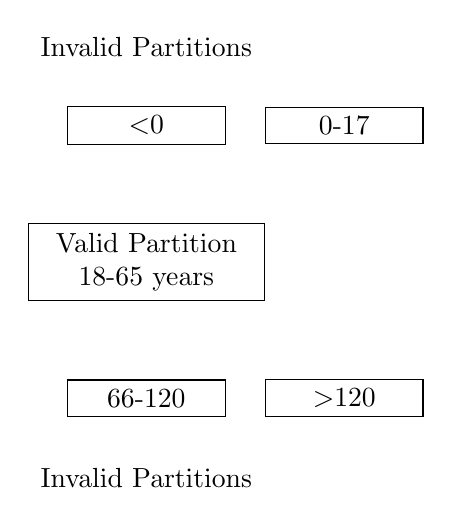
\begin{tikzpicture}[node distance=2cm, auto]
    \node [draw, rectangle, minimum width=3cm, align=center] (valid) {Valid Partition\\ 18-65 years};
    \node [draw, rectangle, above=1cm of valid, minimum width=2cm] (inv1) {$<$0};
    \node [draw, rectangle, right=0.5cm of inv1, minimum width=2cm] (inv2) {0-17};
    \node [draw, rectangle, below=1cm of valid, minimum width=2cm] (inv3) {66-120};
    \node [draw, rectangle, right=0.5cm of inv3, minimum width=2cm] (inv4) {$>$120};
    
    \node [above=2cm of valid] {Invalid Partitions};
    \node [below=2cm of valid] {Invalid Partitions};
\end{tikzpicture}
\captionof{figure}{Equivalence Partitioning Example}
\end{center}

\textbf{Example}: Age validation for job application

\begin{itemize}
    \item \keyword{Valid partition}: 18-65 years
    \item \keyword{Invalid partitions}: $<$0, 0-17, 66-120, $>$120
    \item \keyword{Test cases}: One from each partition (e.g., 25, -5, 10, 70, 130)
\end{itemize}

\textbf{2. Boundary Value Analysis:}

\begin{center}
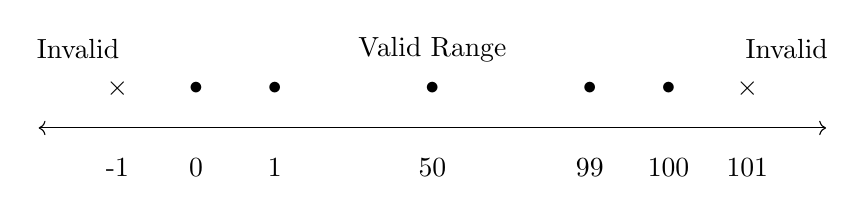
\begin{tikzpicture}[node distance=1.5cm, auto]
    \draw[<->] (0,0) -- (10,0);
    \foreach \x/\label in {1/-1, 2/0, 3/1, 5/50, 7/99, 8/100, 9/101}
        \node at (\x,-0.5) {\label};
    
    \node at (1,0.5) {$\times$};
    \node at (2,0.5) {$\bullet$};
    \node at (3,0.5) {$\bullet$};
    \node at (5,0.5) {$\bullet$};
    \node at (7,0.5) {$\bullet$};
    \node at (8,0.5) {$\bullet$};
    \node at (9,0.5) {$\times$};
    
    \node at (0.5,1) {Invalid};
    \node at (5,1) {Valid Range};
    \node at (9.5,1) {Invalid};
\end{tikzpicture}
\captionof{figure}{Boundary Value Analysis Example}
\end{center}

\textbf{Example}: Student score validation (0-100)

\begin{itemize}
    \item \keyword{Test values}: -1, 0, 1, 50, 99, 100, 101
    \item \keyword{Focus}: Just inside and outside boundaries
    \item \keyword{Rationale}: Most errors occur at boundaries
\end{itemize}

\textbf{Benefits:}

\begin{itemize}
    \item \keyword{Independence}: No programming knowledge required
    \item \keyword{User perspective}: Tests from user's viewpoint
    \item \keyword{Requirement validation}: Verifies functional specifications
\end{itemize}
\end{solutionbox}

\begin{mnemonicbox}
\mnemonic{EBDSUE: Equivalence, Boundary, Decision, State, Use case, Error guessing}
\end{mnemonicbox}

\end{document}
